\beginsong{Flandern in Not}[
    txt={Elsa Laura von Wolzogen}, 
    txtjahr={1917}
    mel={nach einem Totentanzlied aus dem 16. Jahrhundert}, 
    bo={66}, 
    gruen={168}, 
    siru={48}, 
    index={Der Tod reit'},
]

\beginverse
\endverse
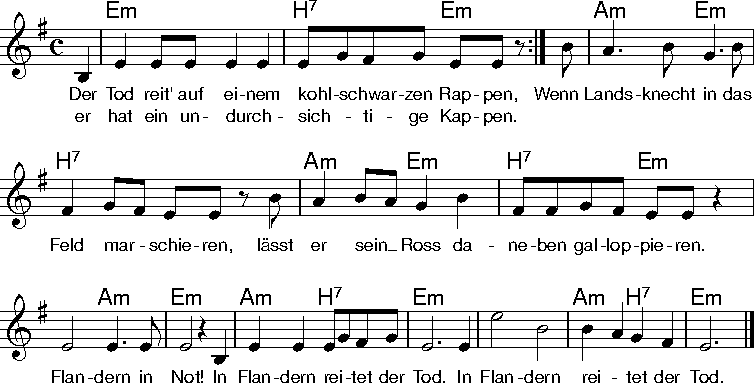
\includegraphics[draft=false, width=1\textwidth]{Noten/Lied044.pdf}	

\beginverse
Der \[Em]Tod reit' auf einem \[H7]lichten \[Em]Schimmel, schön wie ein Cheru\[H7]bin vom \[Em]Himmel,
wenn \[Am]Mädchen \[Em]ihren \[H7]Reigen \[Em]schreiten, will \[Am]er mit \[Em]ihnen im \[H7]Tanze \[Em]gleiten.\newline

\[Am]Falala\[Em]la, \[Am]falala\[Em]la.
\endverse

\beginverse
Der \[Em]Tod kann auch die \[H7]Trommel \[Em]rühren, man kann den Wirbel im \[H7]Herzen \[Em]spüren.
Er \[Am]trommelt \[Em]hell, er \[H7]trommelt \[Em]laut, er \[Am]schlägt auf \[Em]eine \[H7]Toten\[Em]haut.\newline\newpage

Flan\[Am]dern in \[Em]Not! In \[Am]Flandern \[H7]reitet der \[Em]Tod. In Flandern \[Am]rei\[H7]tet der \[Em]Tod.
\endverse

\beginverse
Als ^er den ersten ^Wirbel ge^schlagen, da hat's das Blut vom ^Herzen ge^tragen.
Als ^er den ^zweiten ^Wirbel ^schlug, den ^Landsknecht ^man zu ^Grabe ^trug.\newline

\[Am]Falala\[Em]la, \[Am]falala\[Em]la.
\endverse

\beginverse
Der ^dritte Wirbel ist ^so lang ge^gangen, bis der Landsknecht von Gottes ^Segen em^pfangen.
Der ^dritte ^Wirbel ist ^leis' und ^lind, als ^wiegt eine ^Mutter in ^Schlaf ihr ^Kind.\newline

\[Am]Falala\[Em]la, \[Am]falala\[Em]la.
\endverse

\beginverse
Der ^Tod kann Rappen und ^Schimmel ^reiten, der Tod kann lächelnd im ^Tanze ^schreiten.
Er ^trommelt ^laut, er ^trommelt ^fein: Ge^storben, ge^storben, ge^storben muss ^sein!\newline

Flan\[Am]dern in \[Em]Not! In \[Am]Flandern \[H7]reitet der \[Em]Tod. In Flandern \[Am]rei\[H7]tet der \[Em]Tod.
\endverse

\endsong

\beginscripture{}
1917 versuchten die Alliierten im Ersten Weltkrieg, in Ypern in der belgischen Region Flandern die feindlichen Linien zu durchbrechen. Die ''Dritte Flandernschlacht'' entwickelte sich zur größten Materialschlacht des Krieges.
Das Lied wurde zuerst in der Frontzeitung des Wandervogels veröffentlicht.
\endscripture
